\documentclass[11pt]{article}

\usepackage[utf8]{inputenc}
\usepackage[margin=2cm]{geometry} 
\usepackage{hyperref}
\usepackage{graphicx}
\usepackage{float}
\usepackage{caption}
\usepackage{longtable}
\usepackage{minted}
\usepackage{appendix}
\usepackage{xcolor}
\usepackage{subfig}
\usepackage{bookmark}
\usepackage{array}
\usepackage{multirow}
\usepackage{rotating}

\setlength{\parskip}{1em}
\setlength{\parindent}{0pt}

\begin{document}

% ============ TITLE PAGE ============
\title{\huge Data Mining \& Machine Learning F20DL} 
% \\ {\small{\url{ }}}}
\author{Group 4\\Lewis Wilson, Sam Fay-Hunt, Kamil Szymczak, Chun Man }
\date{\today}
\maketitle

% ============ TABLE OF CONTENTS ============
\newpage
\tableofcontents
\thispagestyle{empty}
\pagebreak
\setcounter{page}{1}
% ============   ============   ============

\newpage
\section{Variation in performance with size of the training and testing sets}

\newpage
\section{Variation in performance with change in the learning paradigm (Decision Trees versus
Neural Nets)}

\newpage
\section{Variation in performance with varying learning parameters in Decision Trees}
\subsection{J48}



\newpage
\subsection{Random Forest}



\newpage
\section{Variation in performance with varying learning parameters in Neural Networks}
\subsection{Linear Classifier}



\newpage
\subsection{Multilayer Perceptron}



\newpage
\section{Variation in performance according to different metrics (TP Rate, FP Rate, Precision,
Recall, F Measure, ROC Area)}

% ============ APPENDICES BEGINNING ============
\pagebreak
\appendix
\appendixpage
\addappheadtotoc
\begin{appendices}

\section{Appendix A}

% =================== J48 Images here ===================



% =================== Random Forest Images here ===================

\newpage
\begin{sidewaysfigure}[h!]
    \caption {Accuracy vs Created - Random Forest} \label{AccVCreatedRF}
    \centering
    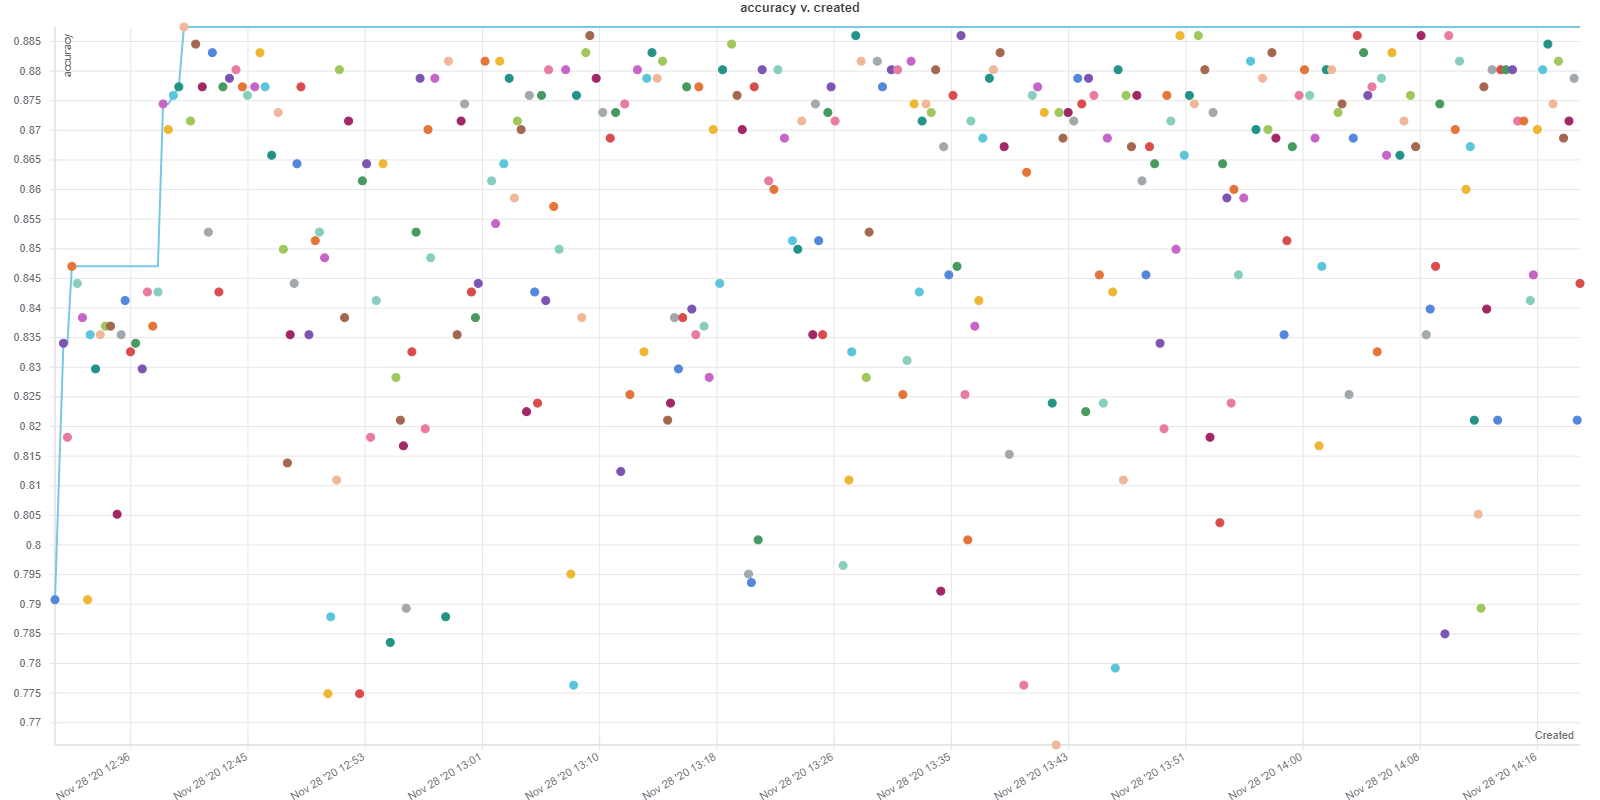
\includegraphics[width = \textwidth, height = \textwidth, keepaspectratio]{Images/RF Accur vs Created.png}
\end{sidewaysfigure}

\newpage
\begin{sidewaysfigure}[h!]
    \caption {Parameter Importance - Random Forest} \label{ParamImportanceRF}
    \centering
    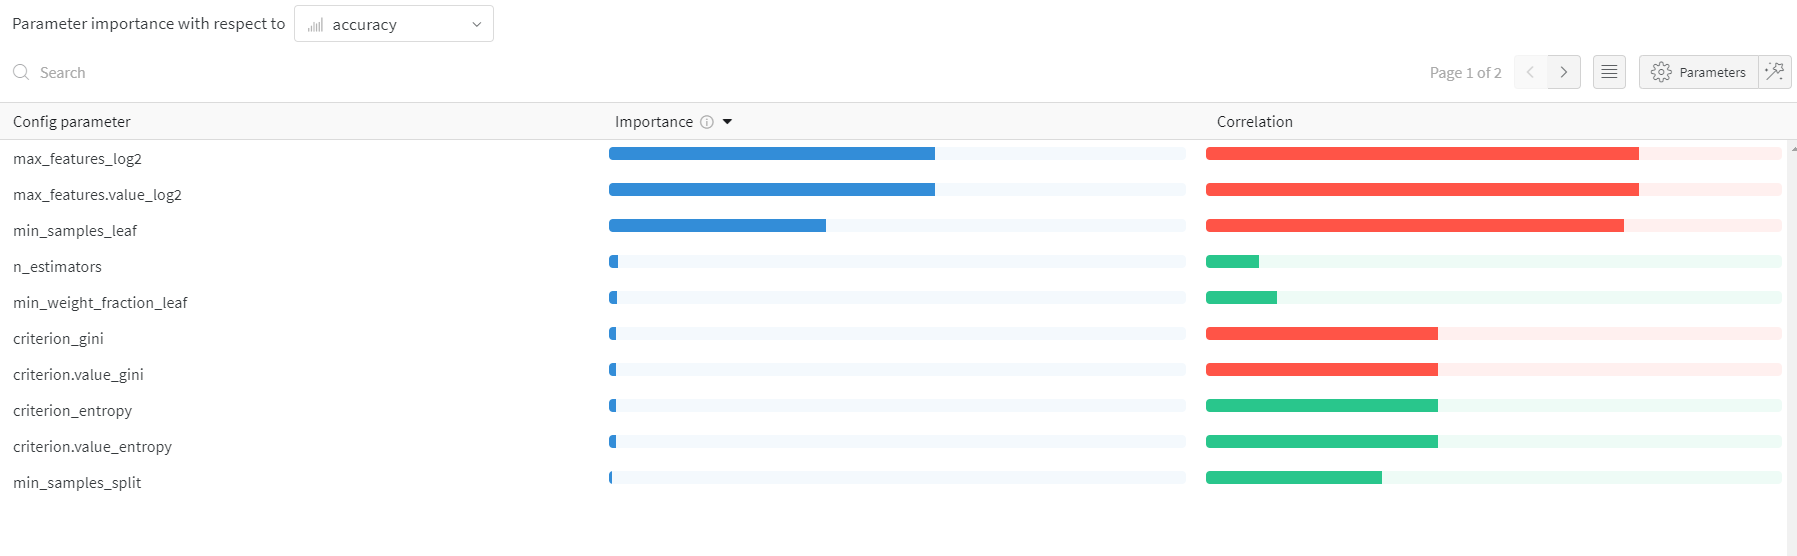
\includegraphics[width = \textwidth, height = \textwidth, keepaspectratio]{Images/RF Parameter Importance.PNG}
\end{sidewaysfigure}

\newpage
\begin{sidewaysfigure}[h!]
    \caption {Random Forest Parameters} \label{ParallelCoordRF}
    \centering
    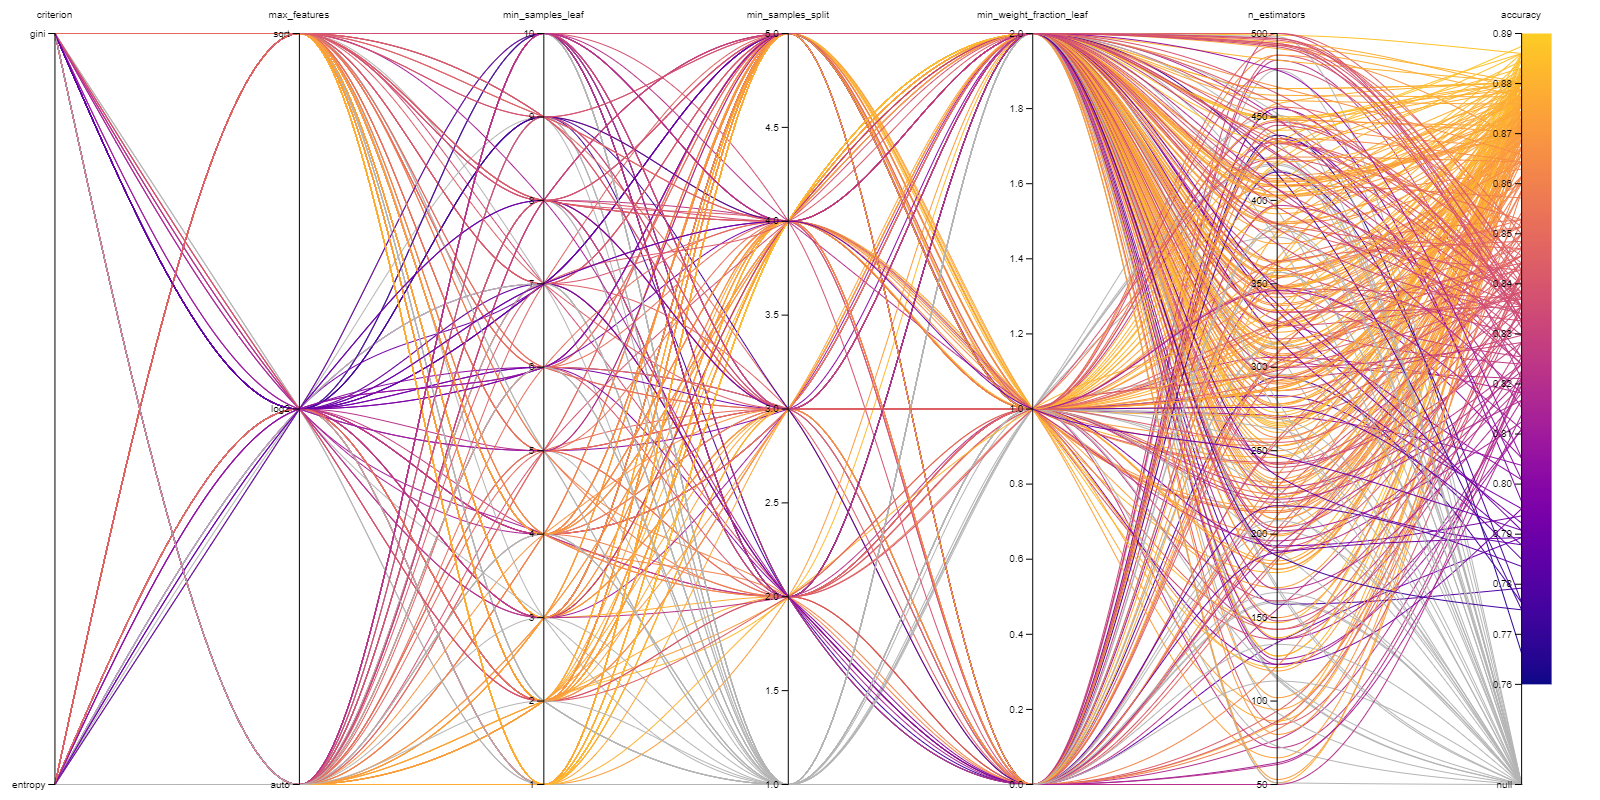
\includegraphics[width = \textwidth, height = \textwidth, keepaspectratio]{Images/RF ParallelCoordGraph.png}
\end{sidewaysfigure}

% =================== Linear Classifier Images here ===================



% =================== Multilayer Perceptron Images here ===================
\end{appendices}

\end{document}